
\section{Durchführung}
\label{sec:Durchführung}
Zur Bestimmung der Leerlaufspannung $U_0$ einer Monozelle wird diese direkt an der Monozelle wie in Abbildung \ref{fig:abbildung1} dargestellt, mit einem Spannungsmesser abgegriffen.
Wie aus Gleichung \eqref{eqn:klemmu} ersichtlich ist, kann bei der Verwendung eines hochohmigen Voltmeter wegen des geringen Stroms $I$ der Term $I R_{\text{i}}$ vernachlässigt werden und es gilt $U_{\text{K}} \approx U_0$.
Zur Berechnung der Leerlaufspannung $U_0$ wird hier allerdings der Innenwiderstand $R_{\text{V}}$ des Voltmeters nicht vernachlässigt. Dieser kann am Messgerät abgelesen werden.

Im Folgenden soll nun die Klemmenspannung $U_{\text{K}}$ der Monozelle in Abhängigkeit vom Belastungsstrom $I$ gemessen werden.
Dazu werden, wie in Abbildung \ref{fig:abbildung2} zu sehen, ein Amperemeter und ein regelbarer Widerstand $R_{\text{a}}$ in Reihe geschaltet mit der Monozelle. Das Voltmeter dient nun zur Messung der Klemmenspannung $U_{\text{K}}$ und bleibt daher weiterhin parallel geschaltet zur Monozelle.
Der Belastungswiderstand $R_{\text{a}}$ wird hierbei variiert im Bereich $0-50 \, \si{\ohm}$.
Es sollen etwa 10 bis 15 Wertepaare der Spannung $U_k$ in Abhängigkeit des Stroms $I$ aufgenommen werden.




\begin{figure}
\centering
\begin{subfigure}{0.53\textwidth}
\centering
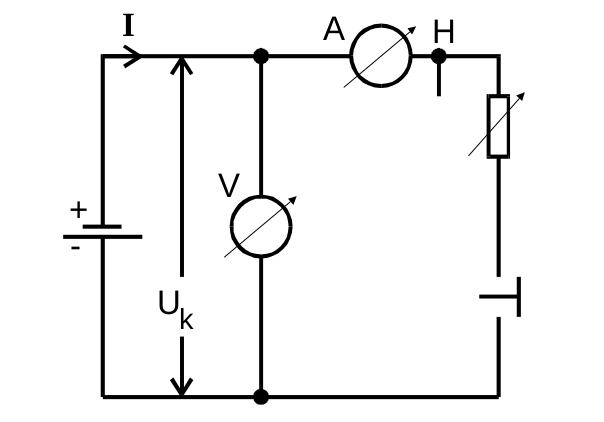
\includegraphics[width=0.9\textwidth]{Bilder/Abbildung2.png}
\caption{Messschaltung zur Bestimmung von $R_i$ und $U_0$ \cite{Anleitung}}
\label{fig:abbildung2}
\end{subfigure}
\begin{subfigure}{0.45\textwidth}
\centering
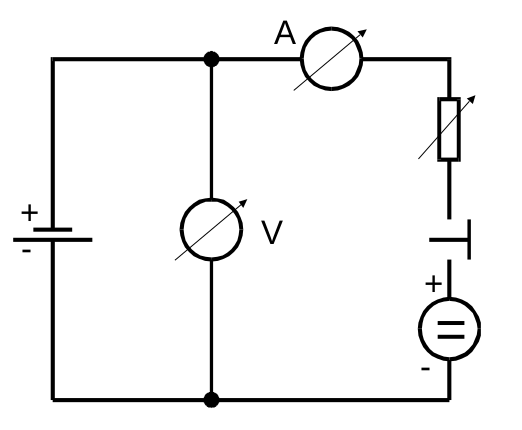
\includegraphics[width=0.9\textwidth]{Bilder/Abbildung3.png}
\caption{Messschaltung \refeq{fig:abbildung2} erweitert um eine Gegenspannung \cite{Anleitung}}
\label{fig:abbildung3}
\end{subfigure}
\end{figure}
In der nächsten Messung soll eine zusätzliche Spannungsquelle in den Schaltkreis eingebracht werden.
Diese soll hierbei $\SI{2}{\volt}$ größer sein als die Leerlaufspannung $U_0$ der Monozelle.
Die neue Spannungsquelle wird, wie in Abbildung \ref{fig:abbildung3} dargestellt, in entgegengesetzer Stromrichtung in Reihe zum Widerstand $R_{\text{a}}$ geschaltet.
Der Strom wird nun also in entgegengesetzter Richtung fließen. Wie bereits in der Messung zuvor wird der Widerstand erneut im Bereich $0-50 \, \si{\ohm}$ variiert und die entsprechenden Werte der Spannung $U_{\text{K}}$ in Abhängigkeit des Strom $I$ notiert.

Nun wird die Monozelle aus der Schaltung ausgebaut und durch einen RC-Generator ersetzt. Wie bereits für die Monozelle soll mit der Schaltung in Abbildung \ref{fig:abbildung2} erneut die Klemmenspannung $U_{\text{K}}$ in Abhängigkeit zu $I$ bestimmt werden. Zunächst wird dazu der 1-$\si{volt}$-Rechteckausgang des RC-Generators verwendet, der Widerstand $R_{\text{a}}$ soll hierbei variiert werden im Bereich $20-250 \, \si{\ohm}$.
In einer weiteren Messung wird der 1-V-Sinusausgang des RC-Generators verwendet, hierbei wird $R_{\text{a}}$ von $0.1-5.0 \, \si{\kilo\ohm}$ variiert.
